% Options for packages loaded elsewhere
\PassOptionsToPackage{unicode}{hyperref}
\PassOptionsToPackage{hyphens}{url}
%
\documentclass[
]{article}
\usepackage{lmodern}
\usepackage{amssymb,amsmath}
\usepackage{ifxetex,ifluatex}
\ifnum 0\ifxetex 1\fi\ifluatex 1\fi=0 % if pdftex
  \usepackage[T1]{fontenc}
  \usepackage[utf8]{inputenc}
  \usepackage{textcomp} % provide euro and other symbols
\else % if luatex or xetex
  \usepackage{unicode-math}
  \defaultfontfeatures{Scale=MatchLowercase}
  \defaultfontfeatures[\rmfamily]{Ligatures=TeX,Scale=1}
\fi
% Use upquote if available, for straight quotes in verbatim environments
\IfFileExists{upquote.sty}{\usepackage{upquote}}{}
\IfFileExists{microtype.sty}{% use microtype if available
  \usepackage[]{microtype}
  \UseMicrotypeSet[protrusion]{basicmath} % disable protrusion for tt fonts
}{}
\makeatletter
\@ifundefined{KOMAClassName}{% if non-KOMA class
  \IfFileExists{parskip.sty}{%
    \usepackage{parskip}
  }{% else
    \setlength{\parindent}{0pt}
    \setlength{\parskip}{6pt plus 2pt minus 1pt}}
}{% if KOMA class
  \KOMAoptions{parskip=half}}
\makeatother
\usepackage{xcolor}
\IfFileExists{xurl.sty}{\usepackage{xurl}}{} % add URL line breaks if available
\IfFileExists{bookmark.sty}{\usepackage{bookmark}}{\usepackage{hyperref}}
\hypersetup{
  pdftitle={Studies of Independent Variables},
  hidelinks,
  pdfcreator={LaTeX via pandoc}}
\urlstyle{same} % disable monospaced font for URLs
\usepackage[margin=0.5cm]{geometry}
\usepackage{color}
\usepackage{fancyvrb}
\newcommand{\VerbBar}{|}
\newcommand{\VERB}{\Verb[commandchars=\\\{\}]}
\DefineVerbatimEnvironment{Highlighting}{Verbatim}{commandchars=\\\{\}}
% Add ',fontsize=\small' for more characters per line
\usepackage{framed}
\definecolor{shadecolor}{RGB}{248,248,248}
\newenvironment{Shaded}{\begin{snugshade}}{\end{snugshade}}
\newcommand{\AlertTok}[1]{\textcolor[rgb]{0.94,0.16,0.16}{#1}}
\newcommand{\AnnotationTok}[1]{\textcolor[rgb]{0.56,0.35,0.01}{\textbf{\textit{#1}}}}
\newcommand{\AttributeTok}[1]{\textcolor[rgb]{0.77,0.63,0.00}{#1}}
\newcommand{\BaseNTok}[1]{\textcolor[rgb]{0.00,0.00,0.81}{#1}}
\newcommand{\BuiltInTok}[1]{#1}
\newcommand{\CharTok}[1]{\textcolor[rgb]{0.31,0.60,0.02}{#1}}
\newcommand{\CommentTok}[1]{\textcolor[rgb]{0.56,0.35,0.01}{\textit{#1}}}
\newcommand{\CommentVarTok}[1]{\textcolor[rgb]{0.56,0.35,0.01}{\textbf{\textit{#1}}}}
\newcommand{\ConstantTok}[1]{\textcolor[rgb]{0.00,0.00,0.00}{#1}}
\newcommand{\ControlFlowTok}[1]{\textcolor[rgb]{0.13,0.29,0.53}{\textbf{#1}}}
\newcommand{\DataTypeTok}[1]{\textcolor[rgb]{0.13,0.29,0.53}{#1}}
\newcommand{\DecValTok}[1]{\textcolor[rgb]{0.00,0.00,0.81}{#1}}
\newcommand{\DocumentationTok}[1]{\textcolor[rgb]{0.56,0.35,0.01}{\textbf{\textit{#1}}}}
\newcommand{\ErrorTok}[1]{\textcolor[rgb]{0.64,0.00,0.00}{\textbf{#1}}}
\newcommand{\ExtensionTok}[1]{#1}
\newcommand{\FloatTok}[1]{\textcolor[rgb]{0.00,0.00,0.81}{#1}}
\newcommand{\FunctionTok}[1]{\textcolor[rgb]{0.00,0.00,0.00}{#1}}
\newcommand{\ImportTok}[1]{#1}
\newcommand{\InformationTok}[1]{\textcolor[rgb]{0.56,0.35,0.01}{\textbf{\textit{#1}}}}
\newcommand{\KeywordTok}[1]{\textcolor[rgb]{0.13,0.29,0.53}{\textbf{#1}}}
\newcommand{\NormalTok}[1]{#1}
\newcommand{\OperatorTok}[1]{\textcolor[rgb]{0.81,0.36,0.00}{\textbf{#1}}}
\newcommand{\OtherTok}[1]{\textcolor[rgb]{0.56,0.35,0.01}{#1}}
\newcommand{\PreprocessorTok}[1]{\textcolor[rgb]{0.56,0.35,0.01}{\textit{#1}}}
\newcommand{\RegionMarkerTok}[1]{#1}
\newcommand{\SpecialCharTok}[1]{\textcolor[rgb]{0.00,0.00,0.00}{#1}}
\newcommand{\SpecialStringTok}[1]{\textcolor[rgb]{0.31,0.60,0.02}{#1}}
\newcommand{\StringTok}[1]{\textcolor[rgb]{0.31,0.60,0.02}{#1}}
\newcommand{\VariableTok}[1]{\textcolor[rgb]{0.00,0.00,0.00}{#1}}
\newcommand{\VerbatimStringTok}[1]{\textcolor[rgb]{0.31,0.60,0.02}{#1}}
\newcommand{\WarningTok}[1]{\textcolor[rgb]{0.56,0.35,0.01}{\textbf{\textit{#1}}}}
\usepackage{graphicx,grffile}
\makeatletter
\def\maxwidth{\ifdim\Gin@nat@width>\linewidth\linewidth\else\Gin@nat@width\fi}
\def\maxheight{\ifdim\Gin@nat@height>\textheight\textheight\else\Gin@nat@height\fi}
\makeatother
% Scale images if necessary, so that they will not overflow the page
% margins by default, and it is still possible to overwrite the defaults
% using explicit options in \includegraphics[width, height, ...]{}
\setkeys{Gin}{width=\maxwidth,height=\maxheight,keepaspectratio}
% Set default figure placement to htbp
\makeatletter
\def\fps@figure{htbp}
\makeatother
\setlength{\emergencystretch}{3em} % prevent overfull lines
\providecommand{\tightlist}{%
  \setlength{\itemsep}{0pt}\setlength{\parskip}{0pt}}
\setcounter{secnumdepth}{-\maxdimen} % remove section numbering

\title{Studies of Independent Variables}
\author{}
\date{\vspace{-2.5em}11.04.2022}

\begin{document}
\maketitle

\hypertarget{bibliotheken-laden-hilfsfunktion}{%
\section{Bibliotheken laden,
Hilfsfunktion}\label{bibliotheken-laden-hilfsfunktion}}

\begin{Shaded}
\begin{Highlighting}[]
\KeywordTok{library}\NormalTok{(GGally)}

\NormalTok{debug <-}\StringTok{ }\NormalTok{T           }\CommentTok{# debug printout}
\NormalTok{debug <-}\StringTok{ }\NormalTok{F           }\CommentTok{# kein debug printout}
\NormalTok{Log <-}\StringTok{ }\ControlFlowTok{function}\NormalTok{(string) \{}
  \ControlFlowTok{if}\NormalTok{(debug)\{}\KeywordTok{print}\NormalTok{(string)\}  }
\NormalTok{\}}
\end{Highlighting}
\end{Shaded}

\hypertarget{fuxfcr-alle-my-gruppen}{%
\section{Für alle MY Gruppen :}\label{fuxfcr-alle-my-gruppen}}

\begin{itemize}
\tightlist
\item
  Resistenzen.Rmd erzeugte Resistenzen{[}Schicht{]}.csv, diese einlesen
\item
  Variablen plotten und Korrelationen berechnen
\end{itemize}

\hypertarget{inklusive-variablen-hsc0-hsc2}{%
\subsection{``Inklusive'' Variablen
HSC0-HSC2}\label{inklusive-variablen-hsc0-hsc2}}

Um die Anzahl der Variablen und evtl. die Korrelationen zu reduzieren,
habe ich hier wieder zurückgerechnet: Wir haben z.B. 3 = 0+1, also habe
ich im Fall husbandry\_system\_calves = 3 die Variablen HSC0 und HSC1
auf 1 gesetzt.

\begin{Shaded}
\begin{Highlighting}[]
\ControlFlowTok{for}\NormalTok{( Schicht }\ControlFlowTok{in} \KeywordTok{c}\NormalTok{(}\StringTok{"U"}\NormalTok{, }\StringTok{"LE8000"}\NormalTok{,}\StringTok{"GT8000"}\NormalTok{) ) \{     }\CommentTok{# Un-stratisfied /  Less than or Equal to 8000 / Greater Than 8000 }
\NormalTok{  Resistenzen <-}\StringTok{ }\KeywordTok{read.csv}\NormalTok{(}\KeywordTok{paste}\NormalTok{( }\StringTok{"Resistenzen"}\NormalTok{,Schicht,}\StringTok{".csv"}\NormalTok{ , }\DataTypeTok{sep=}\StringTok{""}\NormalTok{ ) )}
\NormalTok{  Resistenzen[,}\DecValTok{1}\NormalTok{] <-}\StringTok{ }\OtherTok{NULL}         \CommentTok{# csv schreiben fügt vorne Index-Spalte an; diese entfernen             }
  \ControlFlowTok{if}\NormalTok{(debug)\{}\KeywordTok{View}\NormalTok{(Resistenzen)\}}

\NormalTok{  df <-}\StringTok{ }\KeywordTok{data.frame}\NormalTok{(}\DataTypeTok{WM     =}\NormalTok{ Resistenzen}\OperatorTok{$}\NormalTok{WM.group,    }\CommentTok{# unabhängige Variablen extrahieren}
                   \DataTypeTok{OLS    =}\NormalTok{ Resistenzen}\OperatorTok{$}\NormalTok{OLS.group,   }\CommentTok{# incl. Titel kürzen, sonst Platzprobleme ...}
                   \DataTypeTok{IAC    =}\NormalTok{ Resistenzen}\OperatorTok{$}\NormalTok{IAC.group, }
                   \DataTypeTok{HSC0   =}\NormalTok{ Resistenzen}\OperatorTok{$}\NormalTok{HSC0,}
                   \DataTypeTok{HSC1   =}\NormalTok{ Resistenzen}\OperatorTok{$}\NormalTok{HSC1,}
                   \DataTypeTok{HSC2   =}\NormalTok{ Resistenzen}\OperatorTok{$}\NormalTok{HSC2,}
                   \DataTypeTok{MY     =}\NormalTok{ Resistenzen}\OperatorTok{$}\NormalTok{MY, }
                   \DataTypeTok{SCC    =}\NormalTok{ Resistenzen}\OperatorTok{$}\NormalTok{SCC, }
                   \DataTypeTok{CBC    =}\NormalTok{ Resistenzen}\OperatorTok{$}\NormalTok{CBC, }
                   \DataTypeTok{DIA    =}\NormalTok{ Resistenzen}\OperatorTok{$}\NormalTok{DIA)}
  \KeywordTok{print}\NormalTok{(}\KeywordTok{ggpairs}\NormalTok{(df, }\DataTypeTok{title =} \KeywordTok{paste}\NormalTok{(}\StringTok{"group:"}\NormalTok{,Schicht), }\DataTypeTok{upper=}\KeywordTok{list}\NormalTok{(}\DataTypeTok{continuos=}\KeywordTok{wrap}\NormalTok{(}\StringTok{"cor"}\NormalTok{,}\DataTypeTok{size=}\DecValTok{6}\NormalTok{))))}
  \KeywordTok{print}\NormalTok{(}\StringTok{""}\NormalTok{)}
\NormalTok{\}}
\end{Highlighting}
\end{Shaded}

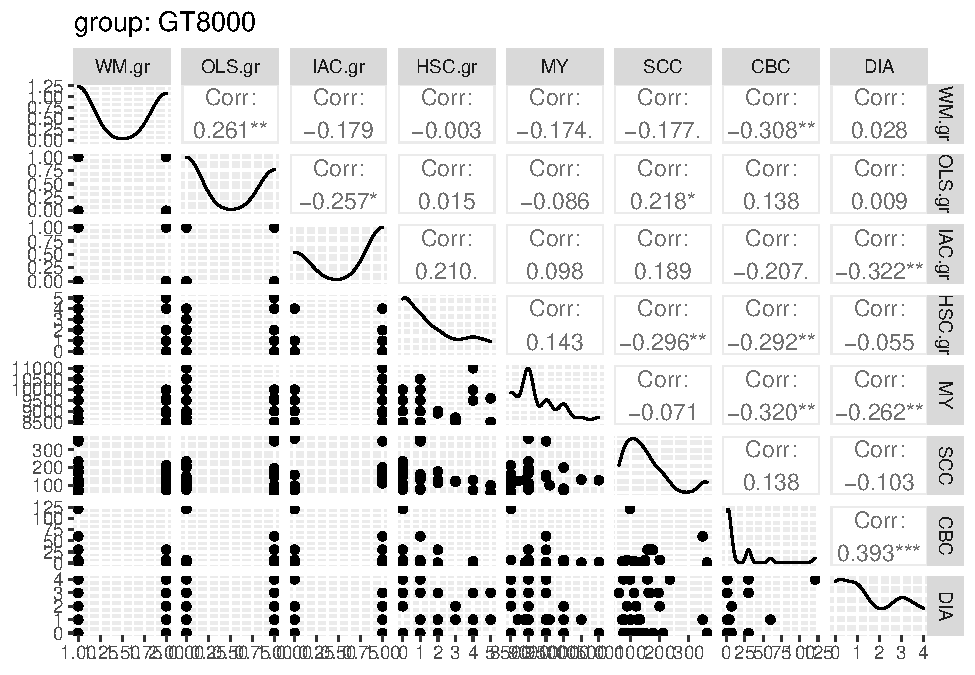
\includegraphics{IndependentVariables_files/figure-latex/unnamed-chunk-2-1.pdf}

\begin{verbatim}
## [1] ""
\end{verbatim}

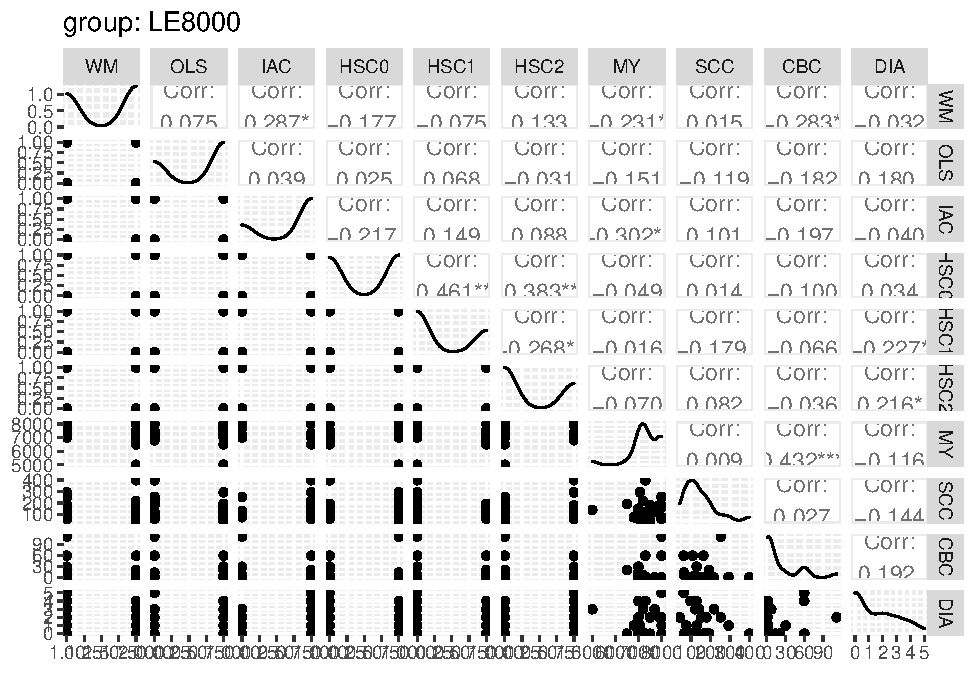
\includegraphics{IndependentVariables_files/figure-latex/unnamed-chunk-2-2.pdf}

\begin{verbatim}
## [1] ""
\end{verbatim}

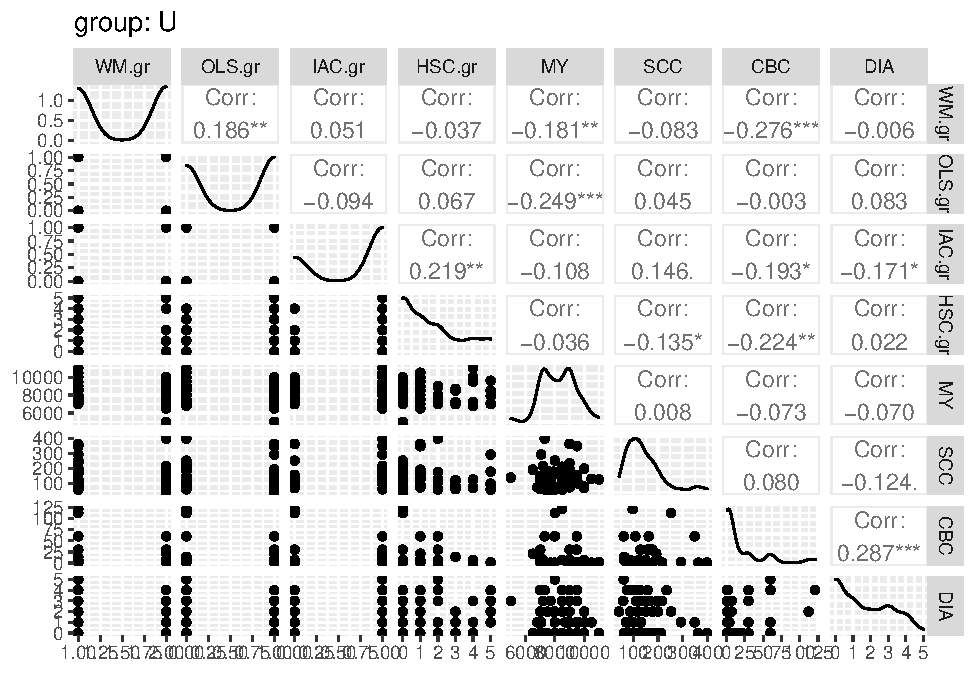
\includegraphics{IndependentVariables_files/figure-latex/unnamed-chunk-2-3.pdf}

\begin{verbatim}
## [1] ""
\end{verbatim}

\hypertarget{linear-depence}{%
\subsubsection{Linear Depence?}\label{linear-depence}}

Linear Dependence implies multicollinearity, so in its presence the
logistic regression would be unreliable.

The correlations with maximum magnitude are

\begin{itemize}
\tightlist
\item
  -53.2\% (HSC0 versus HSC1) in the unstratisfied analysis
\item
  -60.0\% (HSC0 versus HSC1) in the stratisfied analysis MY
  \textgreater{} 8000
\end{itemize}

Due to collinearity problems, it might not be possible to include HSC0
and HSC1 in one multivariate logistic regression.

\hypertarget{outliers}{%
\subsubsection{Outliers?}\label{outliers}}

Einfach zu interpretieren sind nur die plots ohne diskrete Variablen.

In Histogrammen und Streuplots sehe ich einen Ausreisser mit MY = 5000,
das ist Farm 32.

\begin{itemize}
\tightlist
\item
  ist sie als problematisch bekannt?
\item
  das ist aber \emph{kein} Problem für die Regression: MY wird zur
  Schichtung verwendet, nicht als unabhängige Variable
\end{itemize}

\hypertarget{exklusive-variablen-hsc0-hsc5}{%
\subsection{``Exklusive'' Variablen
HSC0-HSC5}\label{exklusive-variablen-hsc0-hsc5}}

Die ursprünglichen Variablen

\begin{Shaded}
\begin{Highlighting}[]
\ControlFlowTok{for}\NormalTok{( Schicht }\ControlFlowTok{in} \KeywordTok{c}\NormalTok{(}\StringTok{"U"}\NormalTok{, }\StringTok{"LE8000"}\NormalTok{,}\StringTok{"GT8000"}\NormalTok{) ) \{     }\CommentTok{# Un-stratisfied /  Less than or Equal to 8000 / Greater Than 8000 }
\NormalTok{  Resistenzen <-}\StringTok{ }\KeywordTok{read.csv}\NormalTok{(}\KeywordTok{paste}\NormalTok{( }\StringTok{"ResistenzenHSC012345/Resistenzen"}\NormalTok{,Schicht,}\StringTok{".csv"}\NormalTok{ , }\DataTypeTok{sep=}\StringTok{""}\NormalTok{ ) )}
\NormalTok{  Resistenzen[,}\DecValTok{1}\NormalTok{] <-}\StringTok{ }\OtherTok{NULL}         \CommentTok{# csv schreiben fügt vorne Index-Spalte an; diese entfernen             }
  \ControlFlowTok{if}\NormalTok{(debug)\{}\KeywordTok{View}\NormalTok{(Resistenzen)\}}

\NormalTok{  df <-}\StringTok{ }\KeywordTok{data.frame}\NormalTok{(}\DataTypeTok{HSC0   =}\NormalTok{ Resistenzen}\OperatorTok{$}\NormalTok{HSC0,}
                   \DataTypeTok{HSC1   =}\NormalTok{ Resistenzen}\OperatorTok{$}\NormalTok{HSC1,}
                   \DataTypeTok{HSC2   =}\NormalTok{ Resistenzen}\OperatorTok{$}\NormalTok{HSC2,}
                   \DataTypeTok{HSC3   =}\NormalTok{ Resistenzen}\OperatorTok{$}\NormalTok{HSC3,}
                   \DataTypeTok{HSC4   =}\NormalTok{ Resistenzen}\OperatorTok{$}\NormalTok{HSC4,}
                   \DataTypeTok{HSC5   =}\NormalTok{ Resistenzen}\OperatorTok{$}\NormalTok{HSC5)}
  \KeywordTok{print}\NormalTok{(}\KeywordTok{ggpairs}\NormalTok{(df, }\DataTypeTok{title =} \KeywordTok{paste}\NormalTok{(}\StringTok{"group:"}\NormalTok{,Schicht), }\DataTypeTok{upper=}\KeywordTok{list}\NormalTok{(}\DataTypeTok{continuos=}\KeywordTok{wrap}\NormalTok{(}\StringTok{"cor"}\NormalTok{,}\DataTypeTok{size=}\DecValTok{6}\NormalTok{))))}
  \KeywordTok{print}\NormalTok{(}\StringTok{""}\NormalTok{)}
\NormalTok{\}}
\end{Highlighting}
\end{Shaded}

\includegraphics{IndependentVariables_files/figure-latex/unnamed-chunk-3-1.pdf}

\begin{verbatim}
## [1] ""
\end{verbatim}

\includegraphics{IndependentVariables_files/figure-latex/unnamed-chunk-3-2.pdf}

\begin{verbatim}
## [1] ""
\end{verbatim}

\includegraphics{IndependentVariables_files/figure-latex/unnamed-chunk-3-3.pdf}

\begin{verbatim}
## [1] ""
\end{verbatim}

Die Korrelationen sind alle negativ, das ist hier klar: nur eine der
Variablen kann 1 sein, die anderen dann alle 0

Korrelationen mit maximalem Betrag:

\begin{itemize}
\tightlist
\item
  -0.410 HSC1 versus HSC0 in der ungeschichteten Analyse
\item
  -0.450 HSC1 versus HSC0 in der Schicht MY \textgreater{} 8000
\end{itemize}

In der Tat etwas kleiner als für die ``inklusiven Variablen''! Wir
sollten diskutieren, welche Variablen besser zu interpretieren sind.

\end{document}
